\documentclass[english,letterpaper]{scrartcl}

\usepackage[breaklinks=true, colorlinks=True, allcolors=blue]{hyperref} 
\usepackage{graphicx}
\usepackage[T1]{fontenc}
\usepackage{booktabs}

\begin{document}
	
\title{New Larval Host Record: \textit{Traminda aventiaria} (Lepidoptera: Geometridae) Feeds on the Critically Endangered Tree, \textit{Serianthes nelsonii} (Leguminosae), on Guam}

\author{Note prepared by Aubrey Moore (\href{mailto://aubreymoore@triton.uog.edu}{aubreymoore@triton.uog.edu})}

\maketitle

In April 2018, Dr. James McConnell discovered a small looper caterpillar feeding on leaves of \textit{Serianthes nelsonii} (Leguminosae), a critically endangered tree species~\cite{Wiles2017}, growing in the Guam Plant Extinction Prevention Program nursery on the University of Guam campus in Mangilao, Guam. He reared the insect into a moth and sent me images which I posted on iNaturalist~\cite{iNat} with a tentative identification of \textit{Thalassodes}.

On December 29 2019, Dr. R. C. Kendrick, responded to the iNaturalist post with a species determination of \textit{Traminda adventiaria} with a follow up comment indicating that Holloway (1997) includes Guam within the geographic range for this species. The first island record for Guam in 1936 was reported by Swezey (1946)~\cite{Swezey1946} (Fig. \ref{fig:swezey}) using the synonym, \textit{Timandra aventiaria}. No other subsequent records for this species are known from Guam.  

\begin{table}[h]
	\centering
	\caption{List of \textit{Traminda aventiaria} larval host plants from Robinson et al. 2010~\cite{Robinson2010}.} 
    \label{tbl:hosts}
	\begin{tabular}{lll}
		\toprule
		Hostplant Family &	Hostplant Name & Country \\
		\midrule
		Gramineae &	& Andaman \& Nicobar Is \\
		Leguminosae & \textit{Acacia} & India \\
		Leguminosae & \textit{Acacia confusa} & Hong Kong \\
		Leguminosae & \textit{Acacia pennata} & India \\
		Leguminosae & \textit{Albizia} & India \\
		Leguminosae & \textit{Albizia} & New Guinea \\
		Umbelliferae & \textit{Oenanthe javanica} & West Malaysia \\
		Leguminosae & \textit{Pithecellobium} & Guam \\
		Leguminosae & \textit{Pithecellobium dulce} & Guam \\
		Rosaceae & \textit{Rosa} & Guam \\
		\bottomrule
	\end{tabular} 
\end{table}


	

\begin{figure}[h]
	\centering
	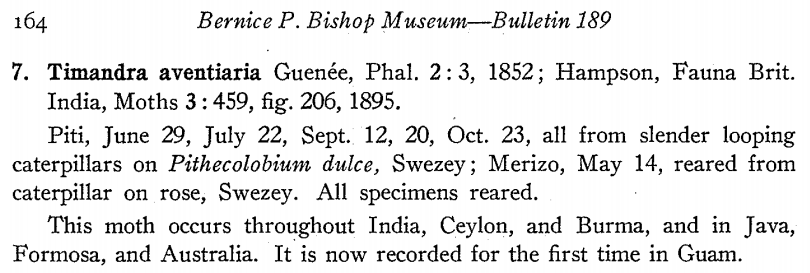
\includegraphics[width=0.9\linewidth]{swezey}
	\caption{First record of \textit{Timandra aventiaria} from Guam. Extracted from Swezey 1946~\cite{Swezey1946}.}
	\label{fig:swezey}
\end{figure}

\begin{figure}[h]
	\centering
	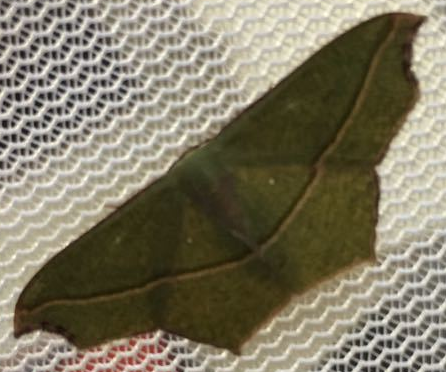
\includegraphics[]{dorsal}
	\caption{\textit{Timandra adventiaria}. Dorsal view.}
	\label{fig:swezey}
\end{figure}

\begin{figure}[h]
	\centering
	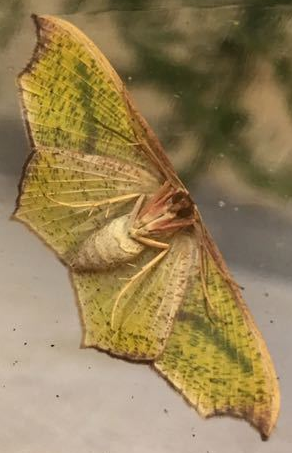
\includegraphics[]{ventral}
	\caption{\textit{Timandra adventiaria} Ventral view.}
	\label{fig:swezey}
\end{figure}

\clearpage

\begin{thebibliography}{1}	
	
	\bibitem{Swezey1946} Swezey, O.H. 1946. Lepidoptera: Geometridae, Arctiidae, Agrotidae and Pyralidae of Guam. In Insects of Guam II, Bernice P. Bishop Museum Bulletin 189, O.H. Swezey, editor. Available online at \url{http://hbs.bishopmuseum.org/pubs-online/pdf/b189p163-185.pdf}. (Accessed 2020-01-01).
	
	\bibitem{iNat} iNaturalist 2018. Observation 11356300. Available online at  \url{https://www.inaturalist.org/observations/11356300}. (Accessed 2020-01-01).
	
	\bibitem{Holloway1997} J.D.Holloway, J.D. 1997. The Moths of Borneo 10. Malayan Nature Journal. Available 0nline at
	\url{http://www.mothsofborneo.com/part-10/timandrini/timandrini_3_1.php}. (Accessed 2020-01-01).
	
	\bibitem{Robinson2010} Robinson, G. S., P. R. Ackery, I. J. Kitching, G. W. Beccaloni and L. M. Hernández, 2010. HOSTS - A Database of the World's Lepidopteran Hostplants. Natural History Museum, London. Available online at \url{https://www.nhm.ac.uk/our-science/data/hostplants/search/index.dsml}. (Accessed 2020-01-01).
	
	\bibitem{Wiles2017} Wiles, G. and E. Williams 2017. Serianthes nelsonii . The IUCN Red List of Threatened Species 2017: e.T30437A98715973. \url{http://dx.doi.org/10.2305/IUCN.UK.2017-3.RLTS.T30437A98715973.en.} (Accessed 2020-01-01).
		
	
\end{thebibliography}

\end{document}
~                  